\documentclass[11pt,spanish,listoffigures,listoftables]{tfgetsinf}

\usepackage[utf8]{inputenc}
\usepackage{tikz,pgfgantt,graphicx,subcaption,float,fourier,array,makecell,pifont,amsmath,titz-uml,rotating,titlesec,forest}

\usetikzlibrary{chains,positioning,shadows,babel,trees}

\setcounter{secnumdepth}{4}
\titleformat{\paragraph}
{\normalfont\normalsize\bfseries}{\theparagraph}{1em}{}
\titlespacing*{\paragraph}
{0pt}{3.25ex plus 1ex minus .2ex}{1.5ex plus .2ex}

%% INFO

\title{Desarrollo de una aplicación móvil multiplataforma \\
para la creación y resolución de nonogramas}
\author{Ignacio Ferrer Sanz}
\tutor{Germán Francisco Vidal Oriola}
\curs{2020-2021}

%% KEYWORDS

\keywords{WIP}
         {nonograma, aplicación, móvil, multiplataforma, Flutter, Firebase, TDD, Clean Architecture}   
         {WIP}

%% BEGIN

\begin{document}

%% SUMMARIES

\begin{abstract}[spanish]
    Resulta innegable que el impacto de las aplicaciones multiplataforma está creciendo incesantemente
    en el mundo de las aplicaciones móviles.
    Cada vez aparecen más \textit{frameworks} de desarrollo capaces de, con ciertas limitaciones,
    facilitar la creación de un único aplicativo que pueda ser usado por los principales sistemas operativos móviles, haciendo frente a
    los ya tradicionales desarrollos nativos.

    Por otra parte, el ámbito de los rompecabezas está muy extendido en las principales
    tiendas de aplicaciones móviles: \textit{Google Play} y \textit{App Store}, siendo una
    de las categorías más populares.

    El objetivo de este trabajo ha sido la de plasmar la pasión personal por los \textit{nonogramas}, rompecabezas de
    origen nipón, en un aplicativo móvil para las plataformas \textit{iOS} y \textit{Android}, en forma de un
    \textit{Minimum Valuable Product} (MVP).
    Este \textit{MVP}, no solo se ha centrado en otorgar al usuario un medio digital interactivo con
    el que resolver estos rompecabezas, sino la de brindar al usuario de un servicio con el que crear
    sus propios \textit{nonogramas}. Esta última característica promoverá, en un futuro, la formación de una comunidad de usuarios activos aficionados
    a este tradicional juego de \textit{puzzle}.

    Para ello, la solución será desarrollada mediante el novedoso \textit{framework} de desarrollo
    móvil \textit{Flutter}, junto a su lenguaje principal de desarrollo \textit{Dart}. Durante su
    desarrollo total, se seguirán las bases de la arquitectura hexagonal \textit{Clean Architecture},
    combinada con la metodología \textit{Test Driven Development}, encargada de validar y verificar el
    sistema de principio a fin.

    En cuanto, los servicios \textit{en línea} a usar por el aplicativo, tales como, la autenticación, bases de datos y analíticas, se desempeñarán mediante la plataforma de 
    desarrollo \textit{back-end} \textit{Firebase}.
\end{abstract}
\begin{abstract}[catalan]
WIP
\end{abstract}
\begin{abstract}[english]
WIP
\end{abstract}

\mainmatter

%% CHAPTERS

\chapter{Introducción}

\textit{Descubrir imágenes hechas píxel de situaciones del día a día,
naturaleza, edificios famosos, personas, y cuantas cosas más, esta es la verdadera esencia de
los nonogramas, también conocidos como hanzies, picross o griddlers.}

\section{Contexto y motivación}

\textit{No importa lo complejo que sea resolver un nonograma, la clave de
estos rompecabezas reside en que su resolución pueda efectuarse por simple
lógica.~\cite{dalgety_2017}} Este era el principal propósito de \textit{James Dalgety} y su equipo
de diseñadores, responsables de dar a conocer a occidente este conocido
pasatiempo nipón, impulsado por el arte de la diseñadora \textit{Non Ishida}, más
adelante, responsable de su principal denominación: \textit{"Non"} Ishida y
Dia\textit{"gram"}.

No fue hasta mediados del año 1990, cuando finalmente se dio a conocer los \textit{nonogramas} a escala
mundial, a través de una publicación del periódico británico \textit{The Sunday
Telegraph}. Más adelante, el mismo noticiero adoptó el término bajo el
seudónimo de \textit{griddlers}, publicándolos semanalmente.

A partir de estas publicaciones, se fue difundiendo exponencialmente el famoso puzzle y
se puede encontrar en revistas, otros periódicos y libros. Fue tan notable su
crecimiento que, como otros rompecabezas, alcanzó con prontitud el formato
digital, en forma de sitios web, videojuegos y aplicaciones.

La capacidad creativa que ofrece resulta ilimitada, ya que con tan solo sus
celdas dispuestas en forma de matriz \textit{(filas y columnas)}, permite
representar todo tipo de figuras, siluetas y formas, como si de un lienzo se
tratara. 

Sorprendentemente y a pesar de que nos encontramos en plena era digital, son pocos los
medios que ofrecen una capacidad de creación, más allá del simple
tradicional método del lápiz y papel y así esta herramienta ayuda y otorga al jugador no solo el rol de \textit{resolutor}, sino de \textit{creador},
e impulsa que la cuantía de \textit{nonogramas} a resolver no disminuya.

Un medio digital es ideal para, no solo hacer que esta propiedad de creación sea posible, sino de facilitar su proceso 
y que sea lo más liviano y recreativo posible, de esta forma las aplicaciones móviles, cada vez más conocidas y presentes en nuestra sociedad, constituyen el entorno
perfecto.

Siguiendo esta premisa, lo que sería adecuado es que cualquier usuario pudiera, dentro de lo posible, emplear estos medios
independientemente de cual sean las características técnicas, sistemas operativos y prestaciones de sus dispositivos.

\section{Objetivos}

El presente trabajo explora el mundo de las aplicaciones móviles y propone
una solución software para: i) permitir al usuario resolver \textit{nonogramas} de forma
interactiva ii) dar la oportunidad de crear sus propios puzzles como lo hizo
\textit{James Dalgety} y su equipo y compartirlos con todos los demás usuarios,
promoviendo así una comunidad de entusiastas de este divertido rompecabezas.

Por consiguiente, para el correcto desarrollo y funcionamiento de la aplicación se deben de
cumplir una serie de requerimientos a nivel técnico bien diferenciados:
\begin{itemize}
   \item[$\bullet$] Estudiar y desarrollar una funcionalidad integrada en el aplicativo, con el fin de posibilitar al usuario
   crear y resolver \textit{nonogramas} en un dispositivo móvil, bajo unas variables determinadas, siempre dando prioridad a la experiencia de juego.
   \item[$\bullet$] Implementar un \textit{backend} con el que el aplicativo pueda complementar sus funcionalidades con \textit{servicios en nube},
   tales como la base de datos, sincronización o inicios de sesión.
   \item[$\bullet$] Seguir los principios de \textit{Clean Arquitecture} durante el proceso de desarrollo, implementando patrones de diseño y
   aplicando \textit{suites de test} con el objetivo de aminorar el proceso de mantenimiento.
   \item[$\bullet$] Definir y realizar un MVP \textit{(Mininum Viable Product)}, con el que usuario pueda, en una primera versión,
   hacer uso de sus funciones principales.
\end{itemize}

Finalmente, encontramos requisitos de índole personal, que progresivamente se considerarán como cumplidos durante todo el desarrollo del proyecto,
tales como:

\begin{itemize}
   \item[$\bullet$] Ahondar en el desarrollo de una aplicación móvil, desde su inicio hasta su finalización,
   bebiendo de buenas prácticas y recomendaciones propuestas por artículos, documentaciones y comunidades de desarrolladores.
   \item[$\bullet$] Comprender y profundizar en el extenso mundo de desarrollo de juegos de puzzles, haciendo frente y reduciendo su
   marcada complejidad.
\end{itemize}

\section{Metodología}

El aplicativo resultante, como cualquier otra solución software, debe satisfacer una serie de requerimientos frente un problema
o problemas concretos. %% TODO: Biblio: definición de aplicación
Esta solución podría residir o enfocarse en diferentes plataformas, bajo una perspectiva
tanto de \textit{software} como de \textit{hardware}.

Así mismo, antes de que esté considerada preparada la aplicación para su uso, ha de atravesar por una serie de procesos,
que difieren mucho de un simple desarrollo y en su conjunto reciben el nombre de \textit{System Development Life Cycle (SDLC)},
que corresponden a su ciclo de vida.

\subsection{Ciclo de vida de desarrollo}
Comprender esta serie de procesos sucesivos, junto a los requisitos recién comentados, es definitorio para elegir una metodología ideal,
que sirva como guía para el correcto desarrollo total del producto.

\begin{itemize}
   \item[$\bullet$] \textbf{Planificación}: identificar los requisitos necesarios para la aplicación,
   considerando y comparando otras soluciones disponibles, para así establecer un \textit{target} o perfil de usuario ideal
   para nuestra aplicación, sin entrar en el apartado técnico.
   \item[$\bullet$] \textbf{Análisis}: establecer los requisitos funcionales de la aplicación, recopilando 
   y anticipándose a aquellos que puedan suponer un problema para la evolución del ciclo de vida.
   \item[$\bullet$] \textbf{Diseño}: documentar las, ya definitivas, características, partes y componentes a integrar en el aplicativo.
   \item[$\bullet$] \textbf{Codificación}: seguir los requisitos ya debidamente documentados e implementarlos creando así el aplicativo. 
   \item[$\bullet$] \textbf{Testing}: una vez desarrollada la solución, realizar \textit{suites de tests} con el fin de encontrar o mostrar
   posibles errores y \textit{bugs}. Además de verificar que los requisitos de la fase de diseño están presentes en la solución.  
   \item[$\bullet$] \textbf{Implementación}: desplegar una primera versión de la aplicación y hacerla disponible en las tiendas principales
   de aplicaciones. 
   \item[$\bullet$] \textbf{Mantenimiento}: monitorizar la experiencia de usuario, contemplando y dando solución a posibles errores,
   además de realizar cambios y mejoras en forma de nuevas versiones.
\end{itemize}

Puesto que en el presente trabajo, durante la primera fase de Planificación, los requisitos han sido detectados y establecidos bajo unos tiempos 
y conocimientos concretos, se ha optado por el modelo clásico de \textit{Modelo en Cascada}.

\subsection{Modelo en casacada} %% http://www.umsl.edu/~hugheyd/is6840/waterfall.html

Siguiendo esta metodología, como se mustra en la Figura ~\ref{fig:M1}, se implantaría un modelo secuencial de todas las diferentes fases del 
\textit{SDLC} del aplicativo, 
desde su fase de Planificación hasta su Mantenimiento, como si se tratara de una cascada.

\begin{figure}[h!]
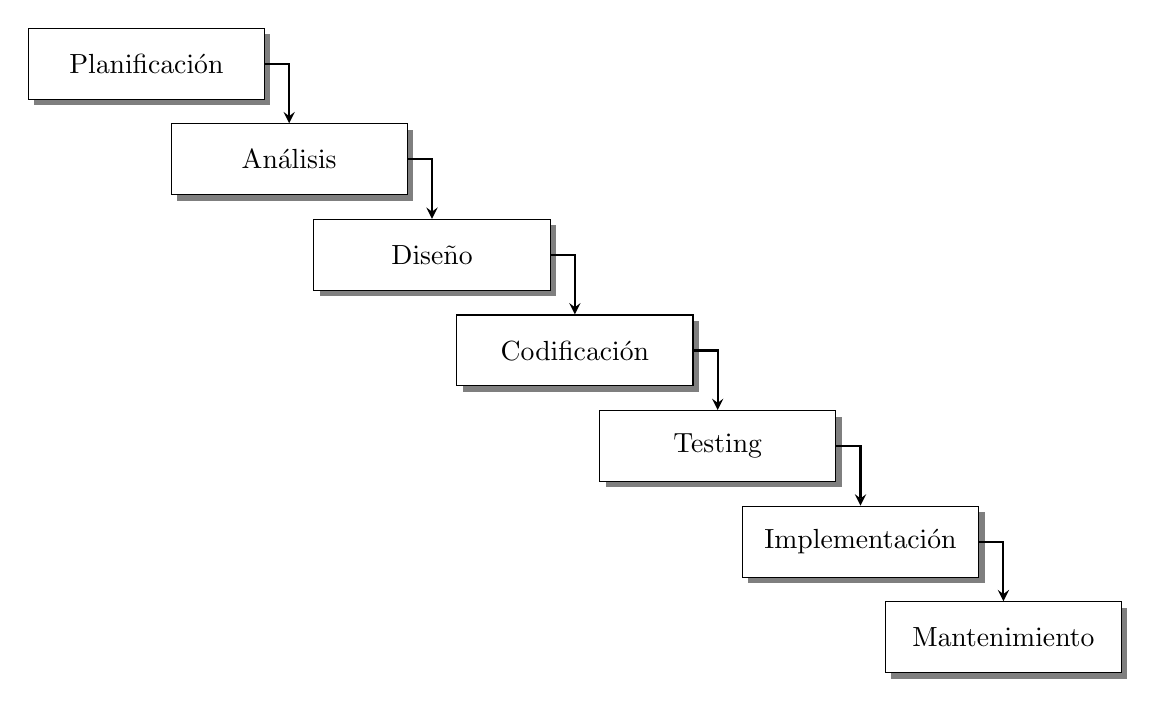
\begin{tikzpicture}[>=stealth,
   node distance = 3mm and -12mm,
     start chain = A going below right,
every node/.style = {draw, text width=28mm, minimum height=9mm, align=center,
                    inner sep=1mm, fill=white, drop shadow={fill=black},  on chain=A}
                  ]
\node {Planificación}; % A-1
\node {Análisis};
\node {Diseño};
\node {Codificación};
\node {Testing};
\node {Implementación};
\node {Mantenimiento};
%
\foreach \i [count=\j] in {2,...,7}
{
 \draw[->, thick] (A-\j) -| (A-\i);
}
\end{tikzpicture}
\caption{Esquema de un Modelo en cascada} \label{fig:M1}
\end{figure}

Sin embargo, como cualquier otra metodología software, es necesario tener en cuenta ciertas consideraciones imprescindibles para el transcurso del proyecto:

\begin{itemize}
   \item[$\bullet$] Como ya se había comentado, es necesario hacer hincapié en las etapas tempranas del modelo, ya que son
   las que van a definir de manera correcta los requisitos de la solución. De forma que, si no están bien establecidos, pueden 
   aparecer problemas en el resto de fases~\cite{wiegers2013software}.
   \item[$\bullet$] Esta metodología carece de iteraciones por lo que no es posible retroceder a las etapas anteriores.
   Hay que cerciorarse de que cada una de las fases se aprueban correctamente, de forma que sea seguro pasar a la
   fase siguiente.
   \item[$\bullet$] En la práctica, es recomendable marcar bien los tiempos de cada fase, marcando estimaciones de cada fase y contrastarlas con
   el tiempo real que ha supuesto realizarlas. Esta especie de monitorización se realizará periódicamente y se puede encontrar 
   en el \autoref{chap:A1}
\end{itemize}

\section{Estructura de la memoria} %%%%% Opcional

El resto de capítulos que conforman la memoria, son los que se resumen a continuación:

\begin{itemize}
   \item[$\bullet$] \textbf{Capítulo 2. Estudio estratégico}: corresponde al conocido apartado \textit{estado del arte}, en el que se realiza una labor 
   de estudio de aquellas soluciones relacionadas con \textit{nonogramas} dentro del mundo digital y que puedan ayudar a la identificación y extracción de requisitos.
   \item[$\bullet$] \textbf{Capítulo 3. Análisis del problema}: en este capítulo se expone la parte de especificación de requisitos,
    identificando aquellos que puedan repercutir negativamente al transcurso del proyecto.
   \item[$\bullet$] \textbf{Capítulo 4. Diseño de la solución}: se muestran las decisiones que se han tomado a nivel de arquitectura, patrones de diseño, 
   y tecnologías empleadas.
   \item[$\bullet$] \textbf{Capítulo 5. Desarrollo de la solución}: se comentan las distintas partes que han compuesto el aplicativo, cómo se comportan y 
   el funcionamiento interno de cada una de ellas, entrando en el apartado técnico.
   \item[$\bullet$] \textbf{Capítulo 6. Pruebas}: se muestran el conjunto de pruebas, que se han desarrollado para la posible identificación de 
   errores y posibles fallos en su ejecución, todas ellas divididas en tipos. 
   \item[$\bullet$] \textbf{Capítulo 7. Implementación y mantenimiento}: se explica el paso que se ha realizado para hacer que el aplicativo sea accesible
   para los usuarios y las medidas para su mantenimiento. 
   \item[$\bullet$] \textbf{Capítulo 8. Manual de uso}: presenta una pequeña demo con el fin de que el usuario se familiarice con el uso de
   la solución, mostrando capturas del mismo.
   \item[$\bullet$] \textbf{Capítulo 9. Conclusión y Trabajo Futuro}: contempla las conclusiones que se han obtenido durante la realización del trabajo y
   las mejoras que se tomarán para siguientes versiones del mismo.
   \item[$\bullet$] \textbf{Apéndices}: se muestran anexos relacionados con análisis de tiempos y apartados relacionados con la codificación del
   la solución y análisis de tiempos.
\end{itemize}

\chapter{Estudio estratégico}
\textit{Los \textit{nonogramas} junto otros gigantes rompecabezas de <<papel y lápiz>> tales como: sudoku, crucigramas, hundir la flota, ahorcado... se han adaptado a
una era en la que está gobernada por las nuevas plataformas tecnológicas. Y más concretamente, en estos tiempos de incertidumbre, confinamientos e incluso ocio han propiciado que estos
puzzles se hagan cada más presentes en nuestras vidas, alejándose una posible obsolescencia.}

\section{Nonogramas en la era Digital}

Pese a que la era Digital ofrece un amplio abanico de medios o plataformas que han incluido y popularizado estos rompecabezas, en
este apartado nos enfocaremos en el de las aplicaciones móviles.

Para que el estudio sea exhaustivo, se explorarán aquellas aplicaciones disponibles en las principales tiendas de aplicaciones para 
las plataformas \textit{Android} e \textit{iOS}, \textit{Google Play} y \textit{App Store} respectivamente.

\subsection{Nonograms Katana}
Nonograms Katana es una aplicación con una remarcada temática nipona, que permite al usuario resolver una gran variedad de \textit{nonogramas},
de una gran variedad de categorías y dimensiones, como se puede comprobar en la Figura~\ref{fig:katana2-1}.

\begin{figure}[H]
   \centering
   \includegraphics[scale=.15]{images/nonokatana1.jpg}
   \caption{Pantalla principal de Nonograms Katana}
   \label{fig:katana1}
 \end{figure}

 Además, como se puede apreciar en la Figura~\ref{fig:katana2-2}, se incluye la resolución de \textit{nonogramas} a color, en el que mediante un selector
 de colores el usuario pinta cada una de las celdas, resolviendo de este modo el \textit{nonograma}.

 \begin{figure}[H]
   \centering
   \begin{subfigure}[b]{0.47\linewidth}
     \includegraphics[width=\linewidth]{images/nonokatana2.jpg}
     \caption{Selector de niveles Nonogramas a color}
     \label{fig:katana2-1}
   \end{subfigure}
   \begin{subfigure}[b]{0.47\linewidth}
     \includegraphics[width=\linewidth]{images/nonokatana3.jpg}
     \caption{Pantalla de resolución de un nivel 20x20 a color}
     \label{fig:katana2-2}
   \end{subfigure}
   \caption{Pantallas de Nonograms Katana con modalidad a color.}
   \label{fig:katana2}
 \end{figure}
 
 El aplicativo sigue la corriente clásica y no permite al usuario resolver los \textit{nonogramas} bajo un número determinado de \textit{vidas} 
 o intentos \textit{(disminuyendo su valor al pulsar sobre celdas erróneas)}, siendo algo tediosa la experiencia de juego, ya que puede acarrear fallos
 durante su resolución.

 Una característica notable de la aplicación es la de permitir al usuario crear sus propios \textit{nonogramas}, compartirlos con la comunidad, y resolver los de
 otros usuarios. Sin embargo, está propiedad no es su principal función y aparece bloqueada si no estás registrado, además de estar limitada por restricciones como los de la 
 Figura~\ref{fig:katana3}.

 El aplicativo presenta la propiedad de multilenguaje, no obstante, este presenta errores en sus traducciones, como se puede comprobar en la figura anteriormente
 citada.

 \begin{figure}[H]
   \centering
   \includegraphics[scale=.175]{images/nonokatana4.jpg}
   \caption{Modal de restricción en publicación en Nonograms Katana}
   \label{fig:katana3}
 \end{figure}
 

\subsection{Nonogram.com - Picture cross number puzzle}

Una de las aplicaciones más descargadas dentro de la categoría puzzle con más de diez millones de descargas en la tienda \textit{Google Play}, 
presenta una interfaz amigable y limpia.

Hace un buen uso de animaciones, destacando la experiencia de juego, algunas bastante remarcables como cuando la que se muestra en la 
Figura~\ref{fig:picture1-2}, en cuanto finalizas un nivel.

\begin{figure}[h!]
   \centering
   \begin{subfigure}[b]{0.45\linewidth}
     \includegraphics[width=\linewidth]{images/picturecross1.png}
     \caption{Pantalla de resolución de un nivel 15x15}
     \label{fig:picture1-1}
   \end{subfigure}
   \begin{subfigure}[b]{0.45\linewidth}
     \includegraphics[width=\linewidth]{images/picturecross2.png}
     \caption{Pantalla de felicitación al resolver el nivel}
     \label{fig:picture1-2}
   \end{subfigure}
   \caption{Pantallas de Nonogram.com}
   \label{fig:picture1}
 \end{figure}

Como característica extra de juego, como se visualiza en la Figura~\ref{fig:picture1-1}, la barra inferior de juego incorpora un botón llamado \textit{Pista}, 
con el que después de ser seleccionado, 
el usuario puede clicar sobre una celda determinada y descubrir si es correcta sin restar una vida, teniendo limitada esta opción a tres usos por nivel.

\begin{figure}[H]
   \centering
   \includegraphics[scale=.25]{images/picturecross3.png}
   \caption{Pantalla de Evento Primavera de Nonogram.com}
   \label{fig:picture2}
 \end{figure}

En el aplicativo, de forma recurrente, aparecen \textit{Eventos} en los que el usuario puede resolver un conjunto de \textit{nonogramas} especiales relacionados
con una temática concreta, representada en la Figura~\ref{fig:picture2}.
 
La solución, como se ha podido comprobar, es de las más completas de las disponibles, no obstante, incluye publicidad excesivamente intrusiva para el usuario,
presente en casi todas sus funcionalidades, que entorpecen la experiencia de juego, incluso llegando a entorpecer al jugador.

\subsection{Nono Infinite}
Este producto destaca por su interfaz \textit{arcade}, con una clara intención de ser dirigida para todos los públicos, constrantando colores muy vivos,
con formas que recuerdan mucho a juegos clásicos para niños, se puede ver reflejado en las Figuras~\ref{fig:infinite1}.

\begin{figure}[h!]
   \centering
   \begin{subfigure}[b]{0.49\linewidth}
     \includegraphics[width=\linewidth]{images/infinite1.png}
     \caption{Pantalla selector de nivel}
     \label{fig:infinite1-1}
   \end{subfigure}
   \begin{subfigure}[b]{0.49\linewidth}
     \includegraphics[width=\linewidth]{images/infinite2.png}
     \caption{Pantalla de resolución de un nivel 5x10}
     \label{fig:infinite1-2}
   \end{subfigure}
   \caption{Pantallas de selección de nivel y juego de Nono Infinite}
   \label{fig:infinite1}
 \end{figure}

Como peculiaridad, presenta \textit{nonogramas} de dimensiones poco usuales que difieren mucho de los clásicos, como el 5x10 presente en la
Figura~\ref{fig:infinite1-2}. Así mismo, permite cambiar la dificultad de los niveles manteniendo las dimensiones del mismo, sin embargo,
esta puede parecer un poco "\textit{artificial"} ya que únicamente aumenta las distancias de las celdas correctas.

Resulta interesante cómo la solución aprovecha el apartado del tutorial, para habituar al usuario de forma interactiva con las reglas clásicas de los 
\textit{nonogramas}, controles del mismo y consejos más avanzados, sobretodo para niveles más complejos, Figura~\ref{fig:infinite2}.

\begin{figure}[H]
   \centering
   \begin{subfigure}[b]{0.4\linewidth}
     \includegraphics[width=\linewidth]{images/infinite3.jpg}
   \end{subfigure}
   \begin{subfigure}[b]{0.4\linewidth}
     \includegraphics[width=\linewidth]{images/infinite4.jpg}
   \end{subfigure}
   \caption{Pantallas de tutorial en Nono Infinite}
   \label{fig:infinite2}
 \end{figure}

 \subsection{Family Crest Nonogram}

 Family Crest Nonogram es un juego que, pese a que no destaque por su apartado gráfico e interfaz de usuario, presenta muchas características que lo diferencian
 del resto de soluciones del género.

 Lo más remarcable de la aplicación es que tenga establecido su uso en modo \textit{landscape} (apaisado), adaptándose al formato de la mayoría de géneros
 de juegos de móvil. Sin embargo, este puede ser un punto negativo para muchos, ya que priva al jugador la esencia de estar jugando a un pasatiempo,
 recordándo más a la de un \textit{videojuego}.

 \begin{figure}[h!]
  \centering
  \begin{subfigure}[b]{0.49\linewidth}
    \includegraphics[width=\linewidth]{images/familycrest1.jpg}
    \caption{Pantalla principal}
    \label{fig:family1-1}
  \end{subfigure}
  \begin{subfigure}[b]{0.49\linewidth}
    \includegraphics[width=\linewidth]{images/familycrest2.png}
    \caption{Pantalla de resolución de un nivel 20x20}
    \label{fig:family1-2}
  \end{subfigure}
  \caption{Pantallas de Family Crest}
  \label{fig:family1}
\end{figure}

No obstante, su experiencia de juego es muy notable, ya que presenta una \textit{cruceta} (para moverse por cada una de las celdas) 
y botones físicos de acción que facilitan un mayor control,
Figura~\ref{fig:family1-2}, además de incorporar una música ambiente que acompaña al usuario cada vez que  está jugando un nivel.

\section{Análisis de las aplicaciones}

Al analizar las aplicaciones enfocadas al submundo de los \textit{nonogramas}, vemos que siguen un patrón de similitudes, que resultan sustanciales 
para el desarrollo de una solución del género rompecabezas, además de ciertas peculiaridades que parecen interesantes para su inclusión en la solución.
Es importante también remarcar y apartar aquellas características que puedan ser perjudiciales para una primera versión de la solución.
A continuación, se muestra un tabla representativa de cada una de las características estudiadas, donde se objetarán su final inclusión en el aplicativo:

\renewcommand\theadalign{b}
\renewcommand\theadfont{\bfseries}
\renewcommand\theadgape{\Gape[1pt]}
\renewcommand\cellgape{\Gape[1pt]}
\newcommand{\cmark}{{\ding{51}}}
\newcommand{\xmark}{{\ding{55}}}
\begin{table}[H]
  \caption{Comparativa de características entre aplicaciones de interés y su inclusión como requisito}
    \begin{tabular}{ | c | c | c | c | c | c |}
      \hline
      \thead{Característica \\ encontrada} & \thead{Nonogram \\ Katana} & \thead{Nonograma.com \\ Picture cross} & \thead{Nono \\ Infinite} & \thead{Family \\ Crest} & \thead{Incluido como \\ requisito} \\
      \hline
      \makecell{Aplicación \\ multiplataforma} &  \cmark  & \cmark  & \xmark & \cmark & \cmark \\
      \hline
      \makecell{Temática \\ especial} &  \cmark  & \xmark  & \cmark & \cmark & \cmark \\
      \hline
      \makecell{Creación \\ nonogramas} &  \cmark*  & \xmark  & \xmark & \xmark & \cmark \\
      \hline
      \makecell{Opción de \\ autoguardado} &  \cmark  & \cmark  & \xmark & \xmark & \cmark* \\
      \hline
      \makecell{Registro de \\ usuario} &  \cmark  & \xmark  & \xmark & \xmark & \xmark \\
      \hline
      \makecell{Sincronización \\de niveles en nube} &  \cmark  & \xmark  & \xmark & \xmark & \cmark \\
      \hline
      \makecell{Juego \\ con \textit{vidas}} &  \xmark  & \cmark  & \xmark & \xmark & \cmark* \\
      \hline
      \makecell{Música \\ ambiente} &  \xmark  & \xmark  & \xmark & \cmark & \xmark \\
      \hline
      \makecell{Botón de \\ pistas} &  \xmark  & \cmark  & \xmark & \xmark & \xmark \\
      \hline
      \makecell{Botones físicos \\ de acción} &  \cmark  & \cmark  & \cmark & \cmark & \xmark \\
      \hline
      \makecell{Variedad de\\ visuales} &  \cmark  & \xmark  & \xmark & \xmark & \cmark \\
      \hline
      \makecell{Multi- \\ idioma} &  \cmark*  & \cmark  & \xmark & \xmark & \cmark \\
      \hline
      \makecell{Eventos \\ especiales} &  \xmark  & \cmark  & \xmark & \xmark & \xmark \\
      \hline
      \makecell{Nonogramas \\ a color} &  \cmark  & \xmark  & \xmark & \xmark & \xmark \\
      \hline
      \makecell{Tutorial \\ de juego} &  \cmark  & \cmark  & \cmark & \xmark & \cmark \\
      \hline
      \makecell{Sección \\ Leaderboard} &  \cmark  & \cmark  & \xmark & \xmark & \xmark \\
      \hline
      \makecell{Selector de \\ niveles} &  \cmark  & \xmark  & \xmark & \cmark & \cmark \\
      \hline
    \end{tabular}
    \label{fig:table1}
\end{table}

La inclusión de las características de la Tabla~\ref{fig:table1} se ven indicadas mediante la siguiente simbología:

\begin{enumerate}
	\item \cmark : Característica incluida en el aplicativo.
	\item \xmark : Característica no incluida en el aplicativo.
	\item \cmark* : Característica incluida en el aplicativo con ciertos matices.
\end{enumerate}

\section{Propuesta}
Visualizando las características reflejadas en la Tabla~\ref{fig:table1} sacamos la siguientes conclusiones de cara a la creación de la primera
versión de la aplicación como producto:

\begin{itemize}
  \item[$\bullet$] Ya que la mayoría de apps estudiadas son multiplataforma, el aplicativo funcionará para ambas plataformas \textit{Android} e \textit{iOS}.
  \item[$\bullet$] Seguirá una temática especial con el fin de diferenciarlas del resto, además de ir alternando entre temas diversos cambiando
  la interfaz de usuario.
  \item[$\bullet$] Tanto la resolución como la creación de los nonogramas será una de las funciones de la solución, sin ningún tipo de restricción.
  \item[$\bullet$] El usuario podrá usar \textit{servicios in-cloud} como: sincronización en nube o acceso a la base de datos sin tener que registrarse.
  \item[$\bullet$] La aplicación tendrá posibilidad multi-idioma, teniendo disponible inglés y español para esta primera versión, sin ningún tipo de errata.
  \item[$\bullet$] Se podrán jugar niveles de \textit{nonogramas} de diferentes dimensiones clásicas, recordando a los de los medios físicos tradicionales,
  previamente explicado su uso por un tutorial intuitivo. 
  \item[$\bullet$] Durante la resolución del nonograma, el usuario podrá resolverlo con una interfaz minimalista, en ausencia de botones físicos,
  además de poder alternar entre resolución con y sin \textit{vidas}.
  \item[$\bullet$] Muchas de las características estudiadas se han tomado como no esenciales y quedarán descartadas para la primera versión.
\end{itemize}

\chapter{Análisis del problema}
\textit{La Ingeniería de Requisitos (IR) es el área más importante de la Ingeniería de Software y posiblemente de todo el ciclo de vida de 
una solución software~\cite{chakraboty2012requirements}.}

\section{?? ???? ???? ? ?? ??}

\tikzumlset{fill usecase=white}
\begin{tikzpicture}
    \begin{umlsystem}[x=4, fill=black!10] {Aplicativo} % empty title
        \umlusecase[name=a,width=1.5cm] {Use case}
        \umlusecase[name=b,x=6,width=2.5cm] {Use case b}
        \umlusecase[name=c,x=6,y=-3,width=2.5cm] {Use case c}
        \umlusecase[name=d,y=-3,width=2.5cm] {Use case d}
    \end{umlsystem}


    \umlactor[y=-1,scale=0.7] {Usuario}

    \umlassoc{Usuario}{a}
    
    % \umlextend{a}{b}
    % \umlinclude{c}{d}

    % manual versions of the above
    \draw [tikzuml dependency style] (a) -- node[above] {$\ll \text{extend} \gg$} (b);
    \draw [tikzuml dependency style] (d) -- node[above] {$\ll \text{include} \gg$} (c);

    % bent association
  \end{tikzpicture}


\chapter{Diseño de la solución}
\textit{El desarrollo de una aplicación multiplataforma es una opción cada vez más a tener en 
cuenta dentro del ámbito del desarrollo móvil~\cite{10.1145/3241739}. La mayor parte de desarrollos
se van a querer destinar a las principales plataformas móviles, 
con el fin de llegar al máximo número de usuarios posibles.
}

\section{Tecnología empleada}
Como se había decidido en el segundo capítulo, la realización de este \textit{MVP} irá dirigido para las
plataformas móviles: \textit{Android} e \textit{iOS}. El desarrollo de un aplicación \textit{nativa} para 
cada sistema, evidentemente, no sería factible, ya que implicaría el doble de esfuerzo en la codificación,
testing y mantenimiento del producto~\cite{10.1145/2480362.2480464}.

Por ello, es necesario el uso de un \textit{framework} de ámbito multiplataforma que nos proporcione un
soporte para ambas plataformas. En este caso, se ha optado por la prometedora herramienta de desarrollo
impulsada por \textit{Google}: \textit{Flutter}.

\subsection{Flutter y Dart}
\textit{Flutter} junto a su lenguaje de programación principal, \textit{Dart}, buscan 
aproximar al usuario la apariencia y rendimiento 
propio al de un desarrollo \textit{nativo}, aprovechando todas las ventajas que proporciona 
un \textit{framework multiplataforma}~\cite{7934674}.

\begin{figure}[H]
    \centering
    \includegraphics[scale=0.45]{images/flutter1.pdf}
    \caption{Diagrama de renderización de \textit{Flutter}\cite{leler2019s}}
    \label{fig:flutter1}
  \end{figure}

Esta relación \textit{apariencia/rendimiento}, la consigue \textit{Flutter} de forma exitosa
\textit{renderizando} directamente sus componentes, 
\textit{widgets}, en un \textit{canvas}, permitiendo visualizar el mismo componente en las diferentes plataformas.
Del mismo modo, realiza la conversión directa de servicios propios, \textit{Platform Channels}, en librerías nativas que
interactúan con las funcionalidades propias del dispositivo~\cite{leler2019s}, 
tal y como se puede visualizar en la Figura \ref{fig:flutter1}.

Esta en una de las razones principales por las que se ha elegido el uso de este herramienta frente a otros 
\textit{frameworks} de desarrollo móvil como: 

\begin{itemize}
    \item[$\bullet$] Los \textit{frameworks interpretados} como: \textit{React Native} y \textit{Vue Native}, 
    que necesitan de una
    capa adicional para realizar la conversión a \textit{componentes nativos}, afectando al rendimiento.
    \item[$\bullet$] Los \textit{frameworks embebidos} como
    \textit{Ionic} que emplea un \textit{WebView} para mostrar los componentes dependiendo de la conexión a 
    Internet del dispositivo.
 \end{itemize}

 \subsection{Firebase}
 Para todas las funcionalidades relacionadas con servicios \textit{en nube}, vistos en la fase de Análisis,
 se empleará la plataforma de desarrollo backend impulsada y recomendada por \textit{Google}: \textit{Firebase}.

Gracias a que \textit{Firebase} presenta una base de datos del tipo \textit{real-time}, permitirá 
la sincronización de los datos durante la ejecución del
aplicativo~\cite{khawas2018application}. Esta característica resulta ideal, ya que
\textit{Flutter} al tratarse de un \textit{framework "declarativo"} no requiere de eventos para
sincronizar los datos, permitiendo al usuario visualizar los datos, en todo momento, sincronizados en pantalla,
sin necesidad de que el usuario realice un \textit{input de refrescar}.

Además, esta, al pertenecer al tipo de las \textit{no relacionales}, presenta ciertos beneficios frente a 
las \textit{relacionales},
a tener en cuenta en la definición de los modelos, tales como flexibilidad, seguridad y rendimiento.

La funcionalidades \textit{in-cloud} del \textit{back-end} de la aplicación final 
quedarán cubiertas por los apartados mostrados en la Tabla \ref{fig:tableFirebase}

\begin{table}[H]
    \centering
    \caption{Funcionalidades \textit{en nube} cubiertas por \textit{Firebase}}
      \begin{tabular}{ | c | c |}
        \hline
        \thead{Funcionalidad} & \thead{Tecnología} \\
        \hline
        \makecell{Autentificación} &  \makecell{\textbf{Firebase Authentication}, permite al usuario el acceso a las funciones de \\ la plataforma
        mediante inicio sesión tradicional \\ (cuenta de correo y contraseña)  o por RRSS.} \\
        \hline
        \makecell{Base de datos} &   \makecell{\textbf{Firebase Firestore}, permite al usuario interactuar mediante \\ funciones CRUD 
        la base de datos del sistema.} \\
        \hline
        \makecell{Analíticas} &  \makecell{\textbf{Firebase Analytics}, monitoriza la experiencia de usuario y extrae\\ estadísticas de cara 
        al lanzamiento de futuras versiones tales como:\\ porcentaje de usuarios libre de errores, número de usuarios activos...} \\
        \hline
      \end{tabular}
      \label{fig:tableFirebase}
  \end{table}

  \subsection{Visual Studio Code}
Como \textit{IDE} de desarrollo se empleará la herramienta \textit{Visual Studio Code}, desarrollado por
\textit{Microsoft}, frente a otros entornos como: \textit{XCode} y \textit{Android Studio}, ya que este dispone
de una gran cantidad de \textit{extensiones o plugins} que facilitan notablemente el proceso de \textit{codificación},
además de estar mejor optimizado para labores de \textit{compilación y depuración.}

\subsection{GitHub}
Se empleará \textit{GitHub} para el \textit{control de versiones}, siguiendo la metodología propias de 
\textit{GitFlow}, en el que tendremos, como se puede visualizar en la Figura~\ref{fig:gitflow1}:
i) una rama \textit{master} para versiones finales del aplicativo,
ii) una rama \textit{develop} en la que aunar y testar las funcionalidades desarrolladas y iii) las ramas
\textit{feature} que se crearán por cada caso de uso a desarrollar.

\begin{figure}[H]
    \centering
    \includegraphics[scale=0.6]{images/gitflow1.pdf}
    \caption{Diagrama del funcionamiento de \textit{GitFlow}}
    \label{fig:gitflow1}
  \end{figure}

Además, nos nutriremos de las buenas prácticas, \textit{librerías} y \textit{repositorios} disponibles en la plataforma,
aprovechando la subida exponencial de la comunidad \textit{Flutter} en este último año, posicionándose
dentro de las tecnologías con más \textit{stars} en el \textit{sitio web}~\cite{gittracker}.

\section{Arquitectura del Sistema}
Una vez definidas las tecnologías que se van a utilizar para el desarrollo de la solución, es importante definir una 
arquitectura que encaje dentro del abanico de requisitos que se desean incluir, además de las funcionalidades que
aportan las tecnologías estudiadas.

Se requiere de una arquitectura de \textit{software} que no tenga tanta complejidad, ya que no se trata de un
proceso industrial y el desarrollo va a ser realizado por una persona, además de estar bien establecida, ya que
no se quiere entorpecer la escalabilidad del sistema, facilitando, de esta forma, las fases de testeo y mantenimiento.

Para un desarrollo con \textit{Flutter} como \textit{framework} de desarrollo \textit{front-end} y \textit{Firebase}
como infraestructura de servicios \textit{back-end}, se empleará, \textit{la arquitectura por capas}, o 
\textit{Layered Architecture} 
una de las más arquitecturas más conocidas y elegidas en entornos de desarrollo móvil~\cite{7053865}.

\subsection{Arquitectura por capas}
El objetivo de esta arquitectura es la de abstraer lo máximo posible los diferentes bloques o componentes que van a
conformar el sistema. 

Empleando la siguiente arquitectura se pretenderá obtener, a corto y largo plazo,  los siguientes beneficios:

\begin{itemize}
  \item[$\bullet$] Componentes que desempeñan una única funcionalidad bien definida.
  \item[$\bullet$] Mayor escalabilidad, favoreciendo la inclusión de nuevas funcionalidades.
  \item[$\bullet$] Facilidad en la identificación de posibles \textit{bugs} o errores relativos a la
  ejecución del aplicativo.
  \item[$\bullet$] Permite la inclusión de \textit{patrones de diseño} en el sistema.
  \item[$\bullet$] Código más legible y fácil de entender.
\end{itemize}

Mediante esta arquitectura es posible dividir el sistema mediante N bloques, para el aplicativo final se ha optado por una
arquitectura dividida en cuatro capas, como se puede visualizar en la Figura~\ref{fig:architecture1}.

\begin{figure}[H]
  \centering
  \includegraphics[scale=0.8]{images/architecture.pdf}
  \caption{Diagrama de \textit{Arquitectura basada en cuatro capas}}
  \label{fig:architecture1}
\end{figure}

A continuación, se comentará la funcionalidad de cada una de las capas, en la Tabla~\ref{fig:tablelayers}:

\begin{table}[H]
  \centering
  \caption{Función de las capas de la arquitectura del sistema}
    \begin{tabular}{ | c | c |}
      \hline
      \thead{Capa} & \thead{Funcionalidad} \\
      \hline
      \makecell{Capa de \\ presentación} &  \makecell{Mediante \textit{widgets} se presentarán todas las vistas
      y componentes\\ que contiene el aplicativo.} \\
      \hline
      \makecell{Capa de \\ negocio} &   \makecell{A partir de \textit{manejadores de estados} se controlarán todos los \\ cambios de
      estado presentes en la capa de \textit{presentación}.} \\
      \hline
      \makecell{Capa de \\ dominio} &  \makecell{Las interfaces \textit{repositorio} servirán de esqueleto \\ para las clases relacionadas con
      la capa de \textit{datos}.} \\
      \hline
      \makecell{Capa de \\ datos} &  \makecell{Implementando las interfaces de la capa de \textit{dominio} se
      obtendrán los \\ datos de fuentes externas como nuestro \textit{back-end} de \textit{Firebase}} \\
      \hline
    \end{tabular}
    \label{fig:tablelayers}
\end{table}

Es importante remarcar que, en algunas arquitecturas como \textit{Clean Arquitecture}, se suele abstraer un nivel más 
la capa de dominio aislándolo del sistema, en forma de paquetes externos, 
con el fin de reutilizarlo en otras soluciones~\cite{9071367}.

\subsection{Manejador de estados}

Es cierto que \textit{Flutter}, para aplicaciones más simples permite \textit{manejar estados} directamente
en la \textit{capa de presentación}, mediante la función \textit{setState()}\cite{flutterState}, sin embargo, para nuestra aplicación y otras soluciones de 
gran envergadura y escalabilidad es importante establecer un 
\textit{manejador de estados}, que esté presente en la capa de \textit{negocio}, que se encargue de:

\begin{itemize}
  \item[$\bullet$] Controlar todos los eventos presentes en el aplicativo 
  para transformarlos en estados y transmitirlos a la capa de \textit{presentación}.
  \item[$\bullet$] Obtener los datos sincronizados transmitidos por la capa de \textit{dominio}.
\end{itemize}

Dentro del gran abanico de librerías e implementaciones que ofrece \textit{Flutter} se ha optado por, como se puede 
visualizar en la Figura~\ref{fig:architecture1}, los 
patrones de diseño:

\begin{itemize}
  \item[$\bullet$] \textbf{Provider}: usado para la \textit{inyección de dependencias} directamente en la capa
  de \textit{presentación} transmitiendo estados a la misma. 
  \item[$\bullet$] \textbf{Patrón BLoC}: empleado para centralizar los cambios de estado, recibiendo \textit{eventos}
   de la capa de \textit{presentación} y transmitiendo \textit{estados} que cambien los componentes de la misma.
\end{itemize}

En la práctica, se empleará la combinación de ambos patrones mediante el paquete \textit{flutter\_bloc}, 
donde se podrán visualizar algunos ejemplos de uso en el siguiente capítulo de \textit{Desarrollo de la solución}.


\chapter{Desarrollo de la solución}
\textit{El desarrollo de aplicaciones móviles resulta desafiante por la gran variedad de dispositivos
móviles con diferentes sistemas operativos, características y tamaños \cite{7021823}. Esta tarea
la suplementa Flutter con sus widgets, permitiendo
desarrollar todo tipo de vistas con un diseño adaptativo para la mayoría de dispositivos.
}

\section{Prototipado de pantallas}
El diseño de la totalidad de pantallas se ha realizado siguiendo las pautas y directrices marcadas por
el estándar \textit{Material Design}. Su gran contenido de iconos, estilos y componentes se ha plasmado,
gracias al paquete \textit{material}, directamente en el aplicativo.

Antes del desarrollo completo de cada una de las pantallas del aplicativo se ha optado por el diseño de
\textit{MockUps}, indicando cada uno de los casos de uso y requisitos funcionales vistos en el Capítulo 
3, indicados por los identificadores del \textit{1 al 21}.

\begin{figure}[H]
    \centering
    \begin{subfigure}[b]{0.38\linewidth}
      \includegraphics[width=\linewidth]{images/screen1.pdf}
    \end{subfigure}
    \begin{subfigure}[b]{0.38\linewidth}
      \includegraphics[width=\linewidth]{images/screen2.pdf}
    \end{subfigure}
    \caption{MockUps Pantalla de Inicio y Selector de niveles clásicos}
    \label{fig:design-1}
\end{figure}

La Pantalla de Inicio será la encargada de proveer al usuario el acceso de todos los casos
de uso y requisitos funcionales disponibles.

La pantalla de Selector de niveles clásicos mostrará todos los niveles disponibles predeterminados del sistema,
muchos de ellos extraídos de los libros \textit{Griddlers}, publicados por el noticiero británico 
\textit{Sunday Telegraph}.
A medida los niveles han sido superados se descubrirá el nombre de la figura que representa, Figura \ref{fig:design-1}.

\begin{figure}[H]
    \centering
    \includegraphics[scale=0.83]{images/screen3.pdf}
    \caption{MockUps Pantalla de niveles online y publicación de nonogramas}
    \label{fig:design-2}
\end{figure}

\begin{figure}[H]
  \centering
  \includegraphics[scale=0.83]{images/screen4.pdf}
  \caption{MockUp Pantalla de resolución de nivel}
  \label{fig:design-3}
\end{figure}

En la Figura \ref{fig:design-3} se puede observar el diagrama de flujo de resolución
de nivel. 
Como se puede apreciar, la apariencia y esencia del rompecabezas es fiel al de los medios tradicionales:

\begin{itemize}
  \item[$\bullet$] Las celdas pintadas representan las celdas que se han seleccionado (con un clic) y
  resultan correctas
  \item[$\bullet$] Aquellas celdas con \textit{equis} son las marcadas  por el
  usuario (con doble clic sobre ella), asegurando que no son correctas.
  \item[$\bullet$] Los bloques de los extremos contienen el número
  de celdas correctas de esa fila o columna, los cuales se van difuminado a medida que se van
  resolviendo por el usuario.
\end{itemize}

El jugador puede abandonar el nivel en cualquier momento guardando su progreso si la opción de autoguardado
está activada. En el instante de resolverlo satisfactoriamente (con al menos una vida) se mostrarán
las características del mismo, y en el caso contrario, la opción de volver a intentarlo.

\begin{figure}[H]
  \centering
  \includegraphics[scale=0.83]{images/screen5.pdf}
  \caption{MockUp Pantalla de ajustes y cuenta}
  \label{fig:design-4}
\end{figure}

En la pantalla se pueden configurar propiedades relativas a: 

\begin{itemize}
  \item[$\bullet$] La experiencia de juego como: la posibilidad de autoguardado y
  el número de vidas.
  \item[$\bullet$] El idioma de la totalidad del sistema, por ahora para este \textit{MVP}, entre español e inglés.
  \item[$\bullet$] La combinación de colores que componen el tema del aplicativo.
\end{itemize}

El usuario puede borrar el progreso de todos sus niveles jugados mediante la opción de borrar
progreso; además de sincronizarlo con el \textit{servicio en nube} desde el apartado cuenta, 
iniciando sesión previamente, Figura \ref{fig:design-4}

\section{Estructura del proyecto}
Es importante que en un desarrollo de software se establezca una estructura propia de la arquitectura elegida,
para mantener una modulabilidad y escalabilidad a nivel de sistema.
Para ello, siguiendo las directrices del modelo \textit{Clean Architecture} se ha definido el siguiente
árbol de directorios:

\definecolor{folderbg}{RGB}{230,230,230}
\definecolor{folderborder}{RGB}{110,144,169}

\def\Size{4pt}
\tikzset{
  folder/.pic={
    \filldraw[draw=folderborder,top color=folderbg!50,bottom color=folderbg]
      (-1.05*\Size,0.2\Size+5pt) rectangle ++(.75*\Size,-0.2\Size-5pt);  
    \filldraw[draw=folderborder,top color=folderbg!50,bottom color=folderbg]
      (-1.15*\Size,-\Size) rectangle (1.15*\Size,\Size);
  }
}
\begin{figure}[H]
\begin{center}
\begin{forest}
  for tree={
    font=\scriptsize\ttfamily,
    grow'=0,
    child anchor=west,
    parent anchor=south,
    anchor=west,
    calign=first,
    inner xsep=7pt,
    edge path={
      \noexpand\path [draw, \forestoption{edge}]
      (!u.south west) +(7.5pt,0) |- (.child anchor) pic {folder} \forestoption{edge label};
    },
    before typesetting nodes={
      if n=1
        {insert before={[,phantom]}}
        {}
    },
    fit=band,
    before computing xy={l=15pt},
  }  
[nonochallenge
  [assets ----imágenes{,} iconos{,} y fuentes.
  ]
  [lib ----código fuente dart.
    [api ----funciones y llamadas Firebase.
    ]
    [common ----archivos globales del sistema.
      [theme  ----temas del aplicativo.
      ]
      [utils  ----funciones de utilidad.
      ]
      [widgets  ----widgets comunes del sistema.
      ]
    ]
    [core ----clases genéricas de funcionalidad.
      [error ----clases error y excepciones.
      ]
      [platform ----detección de conexiones ej:internet.
      ]
      [usecase ----definición casos de uso.
      ]
    ]
    [di ----inyector de dependencias.
    ]
    [features ----funcionalidades del sistema.
      [feature1 ----funcionalidad.
        [data ----capa de datos.
          [datasources ---- comunicación con Firebase y base de datos local.
          ]
          [models ----implementación de las entities con serialización y funciones.
          ]
          [repositories\_impl ----implementación de los repositorios de dominio.
          ]
        ]
        [domain ----capa de dominio.
          [entities ----modelos de datos.
          ]
          [repositories ----definición genérica de repositorio.
          ]
          [usecases ----definición de los casos de uso de la funcionalidad.
          ]  
        ]
        [presentation ----capa de presentación y lógica.
          [bloc ----manejador de estados y capa de lógica.
          ]
          [pages ----pantallas de la característica.
          ]
          [widgets ----componentes que componen las pantallas.
          ]
        ]
      ]
      [... ----más funcionalidades.
      ]
    ]
    [i10n ----archivos de traducción.
    ]
  ]
  [tests ----tests del sistema
    [feature1 ----suites de test de funcionalidad: unitarios{,} lógica y widgets.
    ]
    [...
    ]
  ]
]
\end{forest}
\label{fig:tree-1}
\caption{Estructura de directorios de \textit{nonogramchallenge}}
\end{center}
\end{figure}

\section{Codificación del aplicativo}
El proceso de codificación se ha realizado posteriormente a la creación de \textit{suite de tests} de funcionalidades, siguiendo las pautas y
reglas establecidas por la metodología TDD, proceso documentado en el sexto capítulo.

En el siguiente apartado se explicará el \textit{modus operandi} de la codificación de funcionalidades, acompañado de ejemplos definido 
en el anexo, comenzando por la capa de presentación.
%TODO: ref anexo.

\subsection{Desarrollo de la capa de presentación}
La creación de cada una de las pantallas y sus componentes se ha realizado, como no podría ser de otra forma, a partir de un \textit{árbol de widgets}. 
Para el desarrollo de pantallas se ha optado por usar widgets inmutables, llamados, \textit{stateless}, en contraposición a los de tipo \textit{stateful},
con estado mutable. \cite{10.1007/978-981-15-1465-4_56} 

Esta práctica permitirá que las vistas contengan la mínima lógica posible, pudiendo en un futuro reutilizarlas
en otras funcionalidades del sistema o incluso en otras soluciones.

\begin{figure}[H]
  \centering
  \includegraphics[scale=0.83]{images/treewidgets.pdf}
  \caption{Árbol de widgets Pantalla de Resolución de nivel}
  \label{fig:tree-widgets-1}
\end{figure}

En la Figura \ref{fig:tree-widgets-1} y Anexo \ref{cap:anexo1-1} se puede visualizar el \textit{árbol de widgets} de la pantalla de resolución de nivel, los cuales
se ``construyen'' mediante el método \textit{build()}.

Esta vista contiene algunos widgets de interés que se han usado para mejorar la experiencia de usuario como:
\begin{itemize}
  \item[$\bullet$] \textit{SafeArea}: contenedor que acopla la pantalla en el caso que el dispositivo contenga elementos físicos como \textit{notch}, 
  statusbar, marcos de pantalla redondeados...
  \item[$\bullet$] \textit{InteractiveViewer}: permite al usuario realizar gestos como acercar, alejar y mover el rompecabezas 
  para casos en los que el \textit{nonograma} es de grandes dimensiones. 
\end{itemize}

\subsection{Desarrollo de la capa de lógica}
Para implementar la capa de lógica, se usará el paquete \textit{flutter\_bloc}, para ello se definirán todos los 
posibles estados y eventos presentes en dicha funcionalidad y una clase \textit{BLoC} que se encargue de 
``manejar'' el flujo de cambios de estado.

A continuación, se mostrará un diagrama de flujo de estados de la funcionalidad \textit{lista de nonogramas en línea}.

\begin{figure}[H]
  \centering
  \includegraphics[scale=0.83]{images/statesNonoList.pdf}
  \caption{Diagrama de estado de la funcionalidad Lista de nonogramas en línea}
  \label{fig:nonolist-states}
\end{figure}

Cuando el usuario accede a la sección de nonogramas en línea se manejará, por defecto, el estado
inicial \textit{LoadNonoListInitialState}, que a su vez, enviará el evento \textit{LoadingNonoListEvent}.

En cuanto se envíe tal evento, se tramitará el estado \textit{LoadingNonoListState}, mostrando
un widget de carga.

Durante este estado de ``carga'' pedirá al caso de uso \textit{GetNonoListUseCase} la lista de \textit{nonogramas}
disponible en \textit{Firebase}. Tras esta llamada del caso de uso, nos puede devolver los siguientes
tipos de objeto:

\begin{itemize}
  \item[$\bullet$] La totalidad de \textit{nonogramas} publicados por la comunidad disponible en \textit{Firebase}.
  \item[$\bullet$] Un objeto de tipo \textit{Failure}, indicando que no se ha podido tramitar la operación 
  debido a por ejemplo un error de conexión o de base de datos.
\end{itemize}

En el caso de devolver la lista de \textit{nonogramas} actualizado con éxito, se manejará el estado
\textit{LoadedNonoListState}, mostrando la lista de \textit{rompecabezas} al usuario y en su defecto el estado 
de \textit{FailedNonoListState}, cargando una vista de error.

\break

\subsection{Desarrollo de la capa de dominio}
El desarrollo de la \textit{capa de dominio} comienza con la definición de casos de uso a usar por el \textit{BLoC},
esta implementación se realiza a partir de la clase genérica \textit{usecase} disponible en el paquete \textit{core}.

Como se ha podido comprobar en la \textit{capa de dominio}, este caso de uso devuelve un objeto
de tipo \textit{Either<Failure,Type>}, indicando que puede devolver el tipo de objeto deseado, \textit{Type}, o en caso contrario,
un objeto de tipo \textit{Failure} debido a un error ocurrido en la llamada del repositorio. Adicionalmente, este caso de uso puede
recibir o no una lista de parámetros a usar por el repositorio, como por ejemplo, el \textit{uid} del usuario.

Este aspecto, puede realizarse gracias al paquete externo \textit{dartz}, dotando a \textit{Dart} de aspectos y 
beneficios propios de los lenguajes funcionales.

Una vez definido el caso de uso se definirán las clases genéricas de \textit{repositorios} y \textit{entities} a usar en la
\textit{capa de datos}.

Siguiendo la funcionalidad de \textit{Lista de nonogramas en línea} se puede mostrar la implementación de su \textit{capa 
de dominio} en el Anexo.

\subsection{Desarrollo de la capa de datos}
El último paso consiste en desarrollar la \textit{capa de datos} de la funcionalidad, comenzará con la definición de los
\textit{modelos} y la \textit{implementación de los repositorios} a partir de las clases genéricas de \textit{entities} y
\textit{repositories} respectivamente, definidas previamente en la \textit{capa de dominio}.

La implementación de estos \textit{repositorios} emplearán clases de tipo \textit{datasource} que establecerán una conexión
con fuentes de datos externas propias del aplicativo como: i) la base de datos local de la solución y ii) el 
servicio \textit{FireStore} propio de \textit{Firebase}.

Esta \textit{implementación del repositorio} se encargará de
devolver un objeto \textit{Left} o \textit{Right} propio del paquete \textit{dartz}, dependiendo del comportamiento de 
los \textit{datasources} empleados: 

En la funcionalidad citada como ejemplo dichos ejemplos contendrán los siguientes tipos de objeto, tal y como se puede visualizar
en el Anexo:
\begin{itemize}
  \item[$\bullet$] El objeto \textit{Right} contendrá la lista de nonogramas actualizado obtenido por la llamada a \textit{Firebase} realizada por el 
  \textit{datasource}
  \item[$\bullet$] El objeto \textit{Left} contendrá un \textit{Failure} indicando que no se ha podido tramitar la operación 
  debido a por ejemplo un error de conexión o de base de datos.
\end{itemize}

\subsection{Inyección de dependencias}
Por último, con el fin de ``localizar'' cada una de las capas mencionadas y hacerlas accesibles en cada punto del aplicativo,
se empleará el uso de un \textit{Inyector de dependencias}. 

Esta práctica es altamente recomendable, sobretodo, en soluciones de una
extensión importante. Para ello, se definirá en el directorio \textit{di} del sistema raíz \textit{lib} la clase
\textit{injection\_container.dart}, tal y como se puede visualizar en el Anexo.

La definición de esta clase se realizará mediante la librería externa \textit{Get\_It}, uno de los \textit{localizadores de servicios}
más popular. En el se crearán \textit{factories} para "inyectar" los \textit{BLoCs} y \textit{singletons} para el resto de
servicios (\textit{repositories},\textit{use cases}, \textit{datasources} y servicios externos como \textit{Firebase} y \textit{Sqflite}).

\chapter{Pruebas}

\textit{``Los tests en el desarrollo guiado por pruebas (TDD) son los dientes de un engranaje.
Una vez que se desarrolla un test completamente funcional, es seguro que este va a funcionar por y
para siempre.''~\cite{beck2003test}
}

\section{Metodología TDD}
Tal y como se había comentado en el capítulo anterior, el periodo de codificación de cada una de las
funcionalidades ha sido posterior a una fase de creación de \textit{suite de tests automatizados}. 
Este \textit{modus operandi}
es propio de la metodología \textit{Test Driven Development} (TDD), práctica que se ha usado por desarrolladores durante
decadas y que ha ido ganando popularidad como una de las prácticas principales de
la metodología \textit{Extreme Programming}~\cite{1510569}.

\begin{figure}[H]
    \centering
    \includegraphics[scale=0.7]{images/tdd_diagram.pdf}
    \caption{Diagrama de flujo de la metodología TDD}
    \label{fig:tdd-diagram}
\end{figure}

La elección de la arquitectura hexagonal \textit{Clean Architecture} en el proyecto es un aspecto que
facilita notablemente la implementación de la metodología en el proyecto, permitiendo
abstraer completamente los test para poder reutilizarlos incluso en otros casos de uso.

Las pautas de esta metodología sugieren un diagrama de flujo similar al de la \autoref{fig:tdd-diagram},
este flujo de estados se ha aplicado a todas las funcionalidades (\textit{features}) del
proyecto:

\begin{enumerate}
    \item De cara a integrar una nueva funcionalidad en el proyecto, se desarrolla una
    \textit{suite de tests}, obteniendo una idea central y unas pautas más claras de la funcionalidad a desarrollar.
    \item El siguiente paso consiste en ejecutar los tests. De forma evidente se obtiene 
    una serie de resultados fallidos, ya que aún no se ha desarrollado la funcionalidad.
    Las pruebas deben de testar funciones lo más concretas y triviales posibles, además de ser
    completamente independientes unas de otras.
    \item En este momento se desarrolla la funcionalidad, dividida por las capas
    ya comentadas en el anterior capítulo.
    \item Conforme se va desarrollando la funcionalidad la ejecución de los tests
    van adquiriendo valores exitosos. De este modo, se asegura que la las porciones de código desarrolladas
    puedan contener el mínimo número de \textit{bugs}.
    \item Una vez la ejecución de los tests de la funcionalidad tiene ausencia de errores, 
    se procede a la \textit{refactorización} del código (desde cambios de nombres de variables
    hasta desechar posibles elementos innecesarios). Estas sucesivas \textit{refactorizaciones}
    favorecen que el producto esté mantenido de forma constante.
 \end{enumerate}

 Ya enumerados estos pasos, se llega a la conclusión de que la idea central, que alberga esta 
 metodología \textit{TDD}, no se resume como el simple hecho de \textit{testear antes de escribir código}, sino un
 proceso capaz de:

 \begin{itemize}
     \item[$\bullet$] Explorar y comprender mejor la problemática central de la solución antes de comenzar con
     su implementación.
     \item[$\bullet$] Detectar y anticiparse frente a  posibles excepciones o problemas que
     puedan surgir durante el desarrollo.
     \item[$\bullet$] Detectar posibles actualizaciones de requisitos en base a la complejidad
     de una determinada prueba \textit{(retrospectiva)}.
 \end{itemize}

 En la práctica, resulta realmente extensa la cantidad de tipos de pruebas que se pueden emplear para testar una
 solución \textit{software}. \textit{Flutter}, como cualquier otro \textit{framework} de desarrollo, presenta
 numerosas herramientas para favorecer y aligerar esta tarea. Los tipos de pruebas más recurrentes que presenta este entorno
 son: tests de \textit{widgets}, \textit{golden}, \textit{end-to-end}, 
 \textit{integración} y \textit{unitarios}.
 
 Con el fin de obtener la mayor \textit{cobertura de código} posible en el aplicativo, se ha optado por el uso de estos
 tres últimos, además de ser plenamente complementarios. En los siguientes apartados se introducirán y explicarán su uso en el sistema.

 En cuanto al entorno y herramientas que se han empleado para la realización de las pruebas
 son las proporcionadas por el \textit{IDE} de desarrollo \textit{Visual Studio Code}, mediante su modo
 \textit{testing} (\textit{flutter test}).

 Gracias a este entorno se han podido ejecutar todas las baterías de pruebas,
 de forma individual como completa. 

 \subsection{Pruebas unitarias}
 Los tests unitarios son una parte fundamental de cualquier desarrollo
 de \textit{software}, pues son tests automatizados que aseguran el correcto
 funcionamiento de determinados componentes, llamados individualmente como \textit{unidad}.

 Según el volumen ``\textit{Unit Testing: Principles, Practices, and Patterns}'' de \textit{Vladimir Khorikov} (pp. 21) \cite{khorikov2020unit}, un test se considera unitario cuando reúne estas tres características:
 \begin{itemize}
     \item[$\bullet$] Verifica una única funcionalidad.
     \item[$\bullet$] Se crea de forma trivial y rápida.
     \item[$\bullet$] Se desarrolla de forma independiente.
 \end{itemize}

 En este proyecto se han realizado tests de la totalidad de las clases \textit{modelo} y \textit{entidad}, ya que
 son las que va a emplear las funcionalidades del aplicativo final. Entre los más importantes se destaca, como
 no podía ser de otra forma, el \textit{modelo} de la entidad
 \textit{nonograma}, ya que es la que está presente en la mayoría de casos de uso de la solución.

 Mediante el paquete \textit{flutter\_test} se testea un objeto del
 modelo \textit{Nonograma}. Este objeto se instancia en un método \textit{setUp()} con ciertos valores 
 arbitrarios y se testean ciertas casuísticas en forma de \textit{tests}, 
 todos ellos comprendidos en un método \textit{main()}
 que se encarga de ejecutarlos.
 Todos estos \textit{tests} pueden ``agruparse'' en forma \textit{groups}, en el caso de que exista una correlación
 entre cada uno de ellos.

 Algunas de las pruebas unitarias que se han implementado relacionados con el modelo \textit{Nonograma}
 han verificado:

 \begin{itemize}
    \item[$\bullet$] El nombre completo (comprobar que no sea vacío y no contenga carácteres especiales).
    \item[$\bullet$] El número de celdas correctas (comprobar que esté comprendido en el array).
    \item[$\bullet$] Las dimensiones (número de filas y columnas con un formato concreto: 5x5, 10x10,...).
    \item[$\bullet$] La resolución de un nivel concreto (el \textit{nonograma} de la solución sea igual al original).
    \item[$\bullet$] El identificador del \textit{nonograma} sea único con respecto a los otros \textit{nonogramas}.
 \end{itemize}

 \subsection{Pruebas de integración}
 Siguiendo el mismo ejemplar anteriormente citado, un test de \textit{integración} es aquel que no reúne ninguna
 de las tres características, previamente enumeradas, propias de los \textit{tests unitarios}.
 Estos tipos de test cubren las porciones de código relacionadas con los controladores y
 lógicas de negocio.

 En el caso de este aplicativo, las pruebas de integración se encargarán de cubrir y testar todos los posibles comportamientos
 que comprenden los manejadores de estados, las clases \textit{BLoC}.

 En estos tipos de pruebas se inicializa el \textit{BLoC} a probar mediante
 el método \textit{setUp()} y se testea la sucesión de \textit{estados} que emite este mismo
 objeto frente a un determinado \textit{evento}. Toda esta sucesión de \textit{estados} se definen en un \textit{array}
 y se comparan con la cadena de \textit{estados} esperada mediante el método \textit{expect()}.

 Además, los \textit{BLoCs} pueden interactuar con servicios externos a usar por el aplicativo como \textit{bases de datos locales y remotas},
 \textit{pasarelas de pago}, \textit{librerías de terceros}... Y aquí entra en juego un término ampliamente conocido en el mundo del  \textit{testing},
 los \textit{Mocks}.

 Los \textit{mocks} son objetos de ``prueba'' que simulan o imitan ciertos comportamientos
 de objetos reales en un entorno controlado. Con estos tipos de objetos se pueden simular
 todos las casuísticas de una determinado caso de uso, desde excepciones y fallos hasta situaciones
 ideales.
 Todas estos casos en el patrón \textit{BLoC} se pueden traducir en forma de estados.

 El uso de estos \textit{mocks} permitirá el uso de los servicios a emplear por \textit{BLoC} sin
 su concreta implementación en un entorno de \textit{producción}.
 
 Mediante la librería externa \textit{mockito} se permitirá incorporar este tipo de objetos
 en el aplicativo. Cada servicio a simular debe de
 extender de la clase \textit{Mock}, proporcionado por el propio paquete \textit{mockito}.
 En él se inicializan, mediante el método \textit{setUp()}, el \textit{BLoC} a probar junto con
 los servicios a simular mediante \textit{Mocks}.

 Algunas de las pruebas de integración de interés en el aplicativo han verificado las
 siguientes funcionalidades de \textit{BLoCs} relativos a \textit{nonogramas}:

 \begin{itemize}
    \item[$\bullet$] Recibir la lista de \textit{nonogramas} en línea sin errores.
    \item[$\bullet$] Al ``pintar'' una celda comprobar que la celda está dentro de las celdas seleccionadas.
    \item[$\bullet$] La publicación de un \textit{nonograma} concreto sin errores.
    \item[$\bullet$] Comprobar si existe el progreso de la resolución de un nivel si está la opción
    de autoguardado activado.  
    \item[$\bullet$] Al seleccionar la última celda correcta del nivel comprobar que el \textit{nonograma}
    aparece como \textit{resuelto}. 
 \end{itemize}

 \subsection{Pruebas end-to-end}
 Las \textit{pruebas end-to-end}, son las pruebas finales y verifican que
 toda la experiencia de usuario es satisfactoria en un entorno con los servicios reales
 y en conexión y disponibles para el aplicativo. En este momento se definirá si una
 determinada funcionalidad estará preparada para su inclusión en el sistema,
 o en su defecto, requiere un ajuste en el diseño.

 La representación de estos tres tipos de pruebas en el aplicativo se refleja en la \autoref{fig:test-diagram}, en
 esta se puede observar su alcance en este proyecto.

 \begin{figure}[H]
    \centering
    \includegraphics[scale=0.5]{images/testdiagram.pdf}
    \caption{Diagrama de los tipos de pruebas en el aplicativo}
    \label{fig:test-diagram}
\end{figure}

\chapter{Implantación y mantenimiento}
\textit{En un ciclo de vida de un entorno de Integración Continua (CI),
tras una inserción de código en un repositorio, posteriormente revisado por
un tercero, un sistema funcional coge el cambio introducido, comprueba
el código y efectúa una serie de comandos que el cambio es positivo
y no resulta perjudicial para la solución.~\cite{6802994}}

\section{Integración Continua}
Ya que se ha empleado tanto metodología \textit{PXP} como \textit{TDD} para este proyecto,
resultó idóneo el incorporar un aspecto tan positivo como es
la \textit{Integración Continua}.

Como se había comentado anteriormente en la \autoref{sec:git},
la solución se aloja en un repositorio de la plataforma \textit{GitLab}.
Como la mayoría de plataformas de servicios web de control de versiones,
presenta una serie de herramientas propias de prácticas \textit{DevOps} que promueven
el contínuo mantenimiento y seguridad del código, esta propiedad es
posible mediante el servicio \textit{Auto DevOps}.

A través de la opción de \textit{Quality Gate} de \textit{GitLab},
se establecieron ciertas condiciones que debe cumplir cualquier
cambio que se desee introducir a la rama \textit{develop}. Estas comprobaciones
están definidas en un archivo \textit{YAML} en el archivo raíz del
proyecto. De tal forma que cada vez que se realiza un \textit{merge} de una
determinada \textit{feature} o directamente un \textit{commit} hacia la rama
\textit{develop} se ejecutan la totalidad de tests desarrollados. En este
momento, se desarrollan dos vertientes:

\begin{itemize}
    \item[$\bullet$] Si las condiciones fallan no se admite la inserción de los
    cambios a la rama protegida a \textit{develop}, devolviendo un mensaje de error con el test o tests
    fallidos.
    \item[$\bullet$] Si las condiciones se cumplen, se inserta el cambio o los cambios deseados en la rama \textit{develop} con éxito.
\end{itemize}

\section{Actualización del proyecto}
Por último, se quería destacar la adaptación del proyecto de cara a las últimas
versiones de \textit{stable} en \textit{Flutter}, más concretamente la versión \textit{Flutter 2.0.0}.

Esta actualización se estableció el 3 de marzo de 2021 e incorporaba muchas novedades y
cambios, como: soporte para entorno \textit{web}, soporte enfocadas a plataformas:
\textit{macOS}, \textit{Windows} y \textit{Linux}, manejo de anuncios \textit{Add-To-App}
y la incorporación de \textit{null-safety} en \textit{Dart}.

Es esta última característica de la versión la que se quiso incorporar en el proyecto,
esta característica permitiría evitar \textit{aserciones} continuas en el código,
definiendo clases con atributos que pueden llegar a adquirir valores nulos, asegurando
que no ocurren excepciones durante su ejecución.

Para la inclusión de esta última actualización en el proyecto se realizó mediante
una herramienta de migración desarrollada por \textit{Flutter}.
\textit El equipo de {Dart} sugirió una serie de pasos para la inclusión de la característica \textit{null-safety}
en el proyecto~\cite{dartmigrate}.

\begin{enumerate}
    \item Esperar a que los paquetes incluidos en el proyecto adopten la última
    actualización con la etiqueta \textit{null-safety}.
    \item Ejecutar el cliente de migración  
    \item De forma estática analiza el código de tu proyecto.
    \item Prueba que los cambios realizados funcionan.
    \item Si el proyecto está publicado en \textit{pub.dev}, publica el proyecto con
    la etiqueta \textit{null-safety} como una versión \textit{prerelease}.
\end{enumerate}

El resultado de esta migración promovió que todos los paquetes incluidos en el
proyecto estén actualizados con la última actualización \textit{null-safety},
un código más limpio y libre de código innecesario, menos excepciones capturadas relacionadas
con valores nulos.

\section{Publicación}
El último paso sería incluir el aplicativo en las principales tiendas de aplicaciones:
\textit{Google Play Store} y \textit{App Store}, para ello se realizó las siguientes pasos
para ambas plataformas.

\begin{enumerate}
    \item Establecer a nivel de proyecto un id de aplicativo para ambas plataformas, junto a sus
    versiones mínimas y máximas de los sistemas operativos que soporta.
    \item Creación de una cuenta con rol de desarrollador,
    \item Generar una versión \textit{release} (un \textit{App Bundle} para Android y 
    un \textit{IPA} para iOS) firmadas con la cuenta de desarrollador deseada.
    \item Configurar  el entorno, opciones y características propias de las plataformas.
\end{enumerate}

\chapter{Manual de uso}
\textit{En el presente capítulo se mostrará el manual de uso resultante del MVP desarrollado.
Las capturas corresponden al aplicativo compilado en una versión release ejecutado por un dispositivo móvil físico con sistema operativo Android 10.}

\section{Pantalla Inicio}
Una vez iniciada la aplicación, la primera pantalla con la que interactúa el usuario corresponde a la \textit{pantalla principal}.
En ella, si es la primera vez que el usuario inicia el aplicativo, aparece un \textit{pop-up} para elegir
el idioma global del sistema (\autoref{fig:man1-2}).

\begin{figure}[H]
    \centering
    \begin{subfigure}[b]{0.36\linewidth}
      \includegraphics[width=\linewidth]{images/man1.jpeg}
      \caption{Pantalla inicio}
      \label{fig:man1-1}
    \end{subfigure}
    \begin{subfigure}[b]{0.36\linewidth}
      \includegraphics[width=\linewidth]{images/man2.jpeg}
      \caption{Pop-up selector de idioma}
      \label{fig:man1-2}
    \end{subfigure}
    \caption{Pantallas iniciales}
    \label{fig:man1}
  \end{figure}

Mediante los botones del menú, el usuario puede ingresar a cada una de las
secciones que lo componen.

\section{Pantalla Jugar nonogramas clásicos}
Dentro del primer menú de \textit{Jugar} encontraremos una lista de niveles
predefinidos, muchos de ellos son niveles tradicionales extraídos de los publicados por
el noticiario \textit{The Sunday Telegraph}.
En cuanto se resuelve un \textit{nonograma}, se descubre el nombre del
nivel, que representa la figura del \textit{nonograma} resuelto.

El sistema presenta autoguardado que, en el caso de estar activado en \textit{Ajustes},
da la opción de volver al nivel justo en el punto donde lo dejaste por última vez.

Esta característica, como se había comentado anteriormente en el análisis de requisitos es
un imprescindible, ya que es muy recurrente en este tipo de pasatiempos, sobre todo
en la resolución de niveles grandes dimensiones.

En el caso de no seleccionar la opción de cargado, por cualquiera de estas
casuísticas, la resolución del \textit{nonograma} estará completamente
nuevo con un progreso inexistente.

\begin{figure}[H]
    \centering
    \begin{subfigure}[b]{0.45\linewidth}
      \includegraphics[width=\linewidth]{images/man3.jpeg}
      \caption{Pantalla selector de nivel}
      \label{fig:man1-3}
    \end{subfigure}
    \begin{subfigure}[b]{0.45\linewidth}
      \includegraphics[width=\linewidth]{images/man4.jpeg}
      \caption{Pop-up cargar nivel}
      \label{fig:man1-4}
    \end{subfigure}
    \caption{Pop-up cargar nivel}
    \label{fig:man2}
  \end{figure}

  \section{Pantalla Tutorial}
La pantalla de tutorial, explica de forma sencilla el uso del aplicativo,
además de presentar las bases y consejos para la resolución de \textit{nonogramas}.
El usuario podrá manejarse por cada una de las páginas deslizando hacia izquierda
y derecha la información en el idioma establecido.

\begin{figure}[H]
    \centering
    \includegraphics[scale=.3]{images/man5.jpeg}
    \caption{Pantalla de tutorial}
    \label{fig:man3}
  \end{figure}

  \section{Pantalla Resolución de nivel}
  Esta es una de las pantallas principales del aplicativo. Esta, como
  su nombre indica, permite tanto, la resolución de los niveles clásicos, como
  los de en línea creados por otros usuarios. 
  
  Como en los \textit{nonogramas}
  de los medios tradicionales, las matrices de celdas presentan etiquetas en la fila y columna externas,
  indicando el número de celdas correctas divididas en bloques que hay en cada fila o columna.
  Una vez que se van resolviendo las etiquetas van disminuyendo su opacidad indicando su
  resolución.

  El usuario puede seleccionar la celdas correctas haciendo un simple clic sobre ellas.
  De forma similar, se puede realizar doble clic o mantener pulsado las celdas, marcando o desmarcando
  con un aspa las celdas, para indicar
  que esas celdas pueden ser incorrectas y evitar hacer clic sobre ellas.

  Una característica realmente útil, sobre todo para los niveles de mayor dimensiones, tales como el 10x10 de la \autoref{fig:man4},
  el usuario puede acercar o alejar la vista para evitar pulsar una
  celda equivocada. En este modo, se muestra de forma persistente en la barra superior principal, el número de
  vidas que dispone el jugador en todo momento.

  \begin{figure}[H]
    \centering
    \begin{subfigure}[b]{0.45\linewidth}
      \includegraphics[width=\linewidth]{images/man6.jpeg}
      \caption{Nivel 15x15}
      \label{fig:man1-6}
    \end{subfigure}
    \begin{subfigure}[b]{0.45\linewidth}
      \includegraphics[width=\linewidth]{images/man7.jpeg}
      \caption{Nivel 15x15 con zoom}
      \label{fig:man1-7}
    \end{subfigure}
    \caption{Pantalla resolución de nivel}
    \label{fig:man4}
  \end{figure}

  \section{Pantallas En línea}
  Estas pantallas corresponden, como su nombre indica, a las pantallas
  relacionadas con funciones \textit{en línea}. Para hacer uso de las
  siguientes funcionalidades el dispositivo debe de disponer de conexión
  a Internet.

  Una vez se accede a la sección \textit{En línea}, el usuario puede visualizar
  todos los \textit{nonogramas} publicados de la comunidad, dispuestos en
  celdas, cada uno de ellos está representado por su nombre, figura y autor.

  Para poder crear niveles y publicarlos para la comunidad se presionará
  el botón flotante, situado en el borde inferior izquierdo. El siguiente
  paso es rellenar las características y dimensiones del mismo. Finalmente,
  desde la pantalla de \textit{Creación de nonograma}, decidir las celdas
  correctas, ``dibujando'' y formando el \textit{nonograma} a publicar, cuando
  ya esté decidido el diseño presionar el botón de Aceptar (\autoref{fig:man1-9}).


  \begin{figure}[H]
    \centering
    \begin{subfigure}[b]{0.45\linewidth}
      \includegraphics[width=\linewidth]{images/man8.jpeg}
      \caption{Pantalla En Línea}
      \label{fig:man1-8}
    \end{subfigure}
    \begin{subfigure}[b]{0.45\linewidth}
      \includegraphics[width=\linewidth]{images/man9.jpeg}
      \caption{Pantalla Creación de nivel}
      \label{fig:man1-9}
    \end{subfigure}
    \caption{Pantalla de funciones En Línea}
    \label{fig:man5}
  \end{figure}

  \section{Pantallas de Ajustes}
  En estas pantallas se ajustan las diferentes configuraciones del sistema,
  ya comentadas anteriormente como: el número de vidas en partida, el idioma y
  opción de autoguardado.

  La penúltima opción del listado de ajustes
  permite acceder a la pantalla de sincronización, en la que el usuario
  puede iniciar sesión mediante \textit{Google} para cargar su progreso tanto
  en niveles clásicos como en línea, además de permitir publicar \textit{nonogramas}
  para la comunidad.

  La última opción de ``Borrar progreso'' permite, como su nombre indica, borrar
  de forma interna, todos los progresos que se hayan guardado en la base de datos
  local del dispositivo.

  Por último, el aplicativo también dispone de un selector de temas de diseño (Tema) que cambian
  a nivel global la paleta de colores del aplicativo (\autoref{fig:man7}). Estos
  están compuestos de un nombre y tres colores diferenciados, que combinados,
  cambian el aspecto completo del aplicativo.
  
  \begin{figure}[H]
    \centering
    \begin{subfigure}[b]{0.4\linewidth}
      \includegraphics[width=\linewidth]{images/man10.jpeg}
      \caption{Pantalla de Ajustes}
      \label{fig:man1-10}
    \end{subfigure}
    \begin{subfigure}[b]{0.4\linewidth}
      \includegraphics[width=\linewidth]{images/man11.jpeg}
      \caption{Pantalla de sincronización}
      \label{fig:man1-11}
    \end{subfigure}
    \caption{Pantallas de Ajustes}
    \label{fig:man6}
  \end{figure}

  \begin{figure}[H]
    \centering
    \begin{subfigure}[b]{0.22\linewidth}
      \includegraphics[width=\linewidth]{images/man12.jpeg}
    \end{subfigure}
    \begin{subfigure}[b]{0.22\linewidth}
      \includegraphics[width=\linewidth]{images/man13.jpeg}
    \end{subfigure}
    \begin{subfigure}[b]{0.22\linewidth}
        \includegraphics[width=\linewidth]{images/man14.jpeg}
      \end{subfigure}
    \begin{subfigure}[b]{0.22\linewidth}
        \includegraphics[width=\linewidth]{images/man15.jpeg}
      \end{subfigure}
    \caption{Temas visuales globales del aplicativo}
    \label{fig:man7}
  \end{figure}

\chapter{Conclusiones y trabajo futuro}
\textit{La Ingeniería de Software}

\section{Relación del trabajo relacionado con los estudios cursados}


\bibliographystyle{IEEEtranS}
%% \bibliographystyle{plain-spanish}
\bibliography{bibliography.bib}

\APPENDIX

\chapter{Fragmentos de código}

\section{Código de Pantalla de Resolución de Nivel}

\label{cap:anexo1-1}

Este apartado muestra la codificación de la página de la \textit{feature} de Resolución de nivel, (\textit{play\_game}).

\begin{lstlisting}[language=Java]

    import 'package:flutter/material.dart';
    import 'package:flutter_bloc/flutter_bloc.dart';
    
    import '../../../../common/theme/theme.dart';
    import '../widgets/grid_box_view.dart';
    import '../widgets/info_bar_view.dart';
    import '../bloc/play_game_bloc.dart';
    
    class PlayGamePage extends StatelessWidget {
      @override
      Widget build(BuildContext context) {
        var gridBloc = BlocProvider.of<PlayGameBloc>(context);
        var colorSet = ThemeManager.of(context).colorSet;
        return Scaffold(
            appBar: InformationBar(
              mainColor: colorSet.primaryColor,
              sideColor: colorSet.secondaryColor,
            ),
            backgroundColor: colorSet.primaryColor,
            body: SafeArea(
                child: InteractiveViewer(
                    maxScale: 3.6,
                    child: Column(
                        mainAxisAlignment: MainAxisAlignment.spaceEvenly,
                        children: [
                          GridBox(
                            width: gridBloc.width,
                            height: gridBloc.height,
                          ),
                        ]))));
      }
    }
    
    \end{lstlisting}
\cleardoublepage

%% END

\end{document}
